\PassOptionsToPackage{unicode=true}{hyperref} % options for packages loaded elsewhere
\PassOptionsToPackage{hyphens}{url}
\PassOptionsToPackage{dvipsnames,svgnames*,x11names*}{xcolor}
%
\documentclass[16pt,]{krantz}
\usepackage{lmodern}
\usepackage{amssymb,amsmath}
\usepackage{ifxetex,ifluatex}
\usepackage{fixltx2e} % provides \textsubscript
\ifnum 0\ifxetex 1\fi\ifluatex 1\fi=0 % if pdftex
  \usepackage[T1]{fontenc}
  \usepackage[utf8]{inputenc}
  \usepackage{textcomp} % provides euro and other symbols
\else % if luatex or xelatex
  \usepackage{unicode-math}
  \defaultfontfeatures{Ligatures=TeX,Scale=MatchLowercase}
    \setmonofont[Mapping=tex-ansi,Scale=0.7]{Source Code Pro}
\fi
% use upquote if available, for straight quotes in verbatim environments
\IfFileExists{upquote.sty}{\usepackage{upquote}}{}
% use microtype if available
\IfFileExists{microtype.sty}{%
\usepackage[]{microtype}
\UseMicrotypeSet[protrusion]{basicmath} % disable protrusion for tt fonts
}{}
\IfFileExists{parskip.sty}{%
\usepackage{parskip}
}{% else
\setlength{\parindent}{0pt}
\setlength{\parskip}{6pt plus 2pt minus 1pt}
}
\usepackage{xcolor}
\usepackage{hyperref}
\hypersetup{
            pdftitle={Diseño artístico},
            pdfauthor={Ricardo Michel MALLQUI BAÑOS},
            colorlinks=true,
            linkcolor=Maroon,
            filecolor=Maroon,
            citecolor=Blue,
            urlcolor=Blue,
            breaklinks=true}
\urlstyle{same}  % don't use monospace font for urls
\usepackage{color}
\usepackage{fancyvrb}
\newcommand{\VerbBar}{|}
\newcommand{\VERB}{\Verb[commandchars=\\\{\}]}
\DefineVerbatimEnvironment{Highlighting}{Verbatim}{commandchars=\\\{\}}
% Add ',fontsize=\small' for more characters per line
\usepackage{framed}
\definecolor{shadecolor}{RGB}{248,248,248}
\newenvironment{Shaded}{\begin{snugshade}}{\end{snugshade}}
\newcommand{\AlertTok}[1]{\textcolor[rgb]{0.94,0.16,0.16}{#1}}
\newcommand{\AnnotationTok}[1]{\textcolor[rgb]{0.56,0.35,0.01}{\textbf{\textit{#1}}}}
\newcommand{\AttributeTok}[1]{\textcolor[rgb]{0.77,0.63,0.00}{#1}}
\newcommand{\BaseNTok}[1]{\textcolor[rgb]{0.00,0.00,0.81}{#1}}
\newcommand{\BuiltInTok}[1]{#1}
\newcommand{\CharTok}[1]{\textcolor[rgb]{0.31,0.60,0.02}{#1}}
\newcommand{\CommentTok}[1]{\textcolor[rgb]{0.56,0.35,0.01}{\textit{#1}}}
\newcommand{\CommentVarTok}[1]{\textcolor[rgb]{0.56,0.35,0.01}{\textbf{\textit{#1}}}}
\newcommand{\ConstantTok}[1]{\textcolor[rgb]{0.00,0.00,0.00}{#1}}
\newcommand{\ControlFlowTok}[1]{\textcolor[rgb]{0.13,0.29,0.53}{\textbf{#1}}}
\newcommand{\DataTypeTok}[1]{\textcolor[rgb]{0.13,0.29,0.53}{#1}}
\newcommand{\DecValTok}[1]{\textcolor[rgb]{0.00,0.00,0.81}{#1}}
\newcommand{\DocumentationTok}[1]{\textcolor[rgb]{0.56,0.35,0.01}{\textbf{\textit{#1}}}}
\newcommand{\ErrorTok}[1]{\textcolor[rgb]{0.64,0.00,0.00}{\textbf{#1}}}
\newcommand{\ExtensionTok}[1]{#1}
\newcommand{\FloatTok}[1]{\textcolor[rgb]{0.00,0.00,0.81}{#1}}
\newcommand{\FunctionTok}[1]{\textcolor[rgb]{0.00,0.00,0.00}{#1}}
\newcommand{\ImportTok}[1]{#1}
\newcommand{\InformationTok}[1]{\textcolor[rgb]{0.56,0.35,0.01}{\textbf{\textit{#1}}}}
\newcommand{\KeywordTok}[1]{\textcolor[rgb]{0.13,0.29,0.53}{\textbf{#1}}}
\newcommand{\NormalTok}[1]{#1}
\newcommand{\OperatorTok}[1]{\textcolor[rgb]{0.81,0.36,0.00}{\textbf{#1}}}
\newcommand{\OtherTok}[1]{\textcolor[rgb]{0.56,0.35,0.01}{#1}}
\newcommand{\PreprocessorTok}[1]{\textcolor[rgb]{0.56,0.35,0.01}{\textit{#1}}}
\newcommand{\RegionMarkerTok}[1]{#1}
\newcommand{\SpecialCharTok}[1]{\textcolor[rgb]{0.00,0.00,0.00}{#1}}
\newcommand{\SpecialStringTok}[1]{\textcolor[rgb]{0.31,0.60,0.02}{#1}}
\newcommand{\StringTok}[1]{\textcolor[rgb]{0.31,0.60,0.02}{#1}}
\newcommand{\VariableTok}[1]{\textcolor[rgb]{0.00,0.00,0.00}{#1}}
\newcommand{\VerbatimStringTok}[1]{\textcolor[rgb]{0.31,0.60,0.02}{#1}}
\newcommand{\WarningTok}[1]{\textcolor[rgb]{0.56,0.35,0.01}{\textbf{\textit{#1}}}}
\usepackage{longtable,booktabs}
% Fix footnotes in tables (requires footnote package)
\IfFileExists{footnote.sty}{\usepackage{footnote}\makesavenoteenv{longtable}}{}
\usepackage{graphicx,grffile}
\makeatletter
\def\maxwidth{\ifdim\Gin@nat@width>\linewidth\linewidth\else\Gin@nat@width\fi}
\def\maxheight{\ifdim\Gin@nat@height>\textheight\textheight\else\Gin@nat@height\fi}
\makeatother
% Scale images if necessary, so that they will not overflow the page
% margins by default, and it is still possible to overwrite the defaults
% using explicit options in \includegraphics[width, height, ...]{}
\setkeys{Gin}{width=\maxwidth,height=\maxheight,keepaspectratio}
\setlength{\emergencystretch}{3em}  % prevent overfull lines
\providecommand{\tightlist}{%
  \setlength{\itemsep}{0pt}\setlength{\parskip}{0pt}}
\setcounter{secnumdepth}{5}

% set default figure placement to htbp
\makeatletter
\def\fps@figure{htbp}
\makeatother

\usepackage[spanish,es-lcroman]{babel}
\usepackage{booktabs}
\usepackage{graphicx}
\usepackage{amsmath}
\usepackage{makeidx}
\makeindex
%\usepackage{showframe}
%\usepackage[a4paper]{geometry}
%\geometry{verbose,tmargin=3cm,bmargin=3cm,lmargin=3.5cm,rmargin=3cm}
\setlength\parindent{23pt}
\usepackage[singlelinecheck=off]{caption}

\usepackage{times}
\renewcommand{\rmdefault}{ptm}
%\usepackage[lite,subscriptcorrection,nofontinfo,zswash]{mtpro2}

\usepackage{graphicx}

% Determine if the image is too wide for the page.
\makeatletter
\def\ScaleIfNeeded{%
  \ifdim\Gin@nat@width>\linewidth
    \linewidth
  \else
    \Gin@nat@width
  \fi
}
\makeatother

% Resize figures that are too wide for the page.
%\let\oldincludegraphics\includegraphics
%\renewcommand\includegraphics[2][]{%
%  \oldincludegraphics[scale=0.85]{#2}
%}

\usepackage{amsthm}
\makeatletter
\def\thm@space@setup{%
  \thm@preskip=8pt plus 2pt minus 4pt
  \thm@postskip=\thm@preskip
}
\makeatother

\flushbottom 

\frontmatter
\usepackage[]{natbib}
\bibliographystyle{apalike}

\title{Diseño artístico}
\author{Ricardo Michel MALLQUI BAÑOS}
\providecommand{\institute}[1]{}
\institute{Universidad Nacional San Cristóbal De Huamanga}
\date{2021-09-07}

\usepackage{amsthm}
\newtheorem{theorem}{Teorema}[chapter]
\newtheorem{lemma}{Lema}[chapter]
\newtheorem{corollary}{Corolario}[chapter]
\newtheorem{proposition}{Proposición}[chapter]
\newtheorem{conjecture}{Conjectura}[chapter]
\theoremstyle{definition}
\newtheorem{definition}{Definición}[chapter]
\theoremstyle{definition}
\newtheorem{example}{Ejemplo}[chapter]
\theoremstyle{definition}
\newtheorem{exercise}{Ejercicio}[chapter]
\theoremstyle{definition}
\newtheorem{hypothesis}{Hypothesis}[chapter]
\theoremstyle{remark}
\newtheorem*{remark}{Observación}
\newtheorem*{solution}{Solución}
\begin{document}
\maketitle

%\cleardoublepage\newpage\thispagestyle{empty}\null
%\cleardoublepage\newpage\thispagestyle{empty}\null
%\cleardoublepage\newpage
\thispagestyle{empty}
\begin{flushright}
Universidad Nacional San Cristobal de Huamanga

Fisart.cf

Agradecimento a los estudiantes de la ESFAPA FGPA

A la UNSCH


\includegraphics[height=3cm]{U.pdf}
\end{flushright}
%\setlength{\abovedisplayskip}{-5pt}
%\setlength{\abovedisplayshortskip}{-5pt}

{
\hypersetup{linkcolor=}
\setcounter{tocdepth}{2}
\tableofcontents
}
\listoftables
\listoffigures
\newcommand{\N}{\mathbb{N}}
\newcommand{\R}{\mathbb{R}}
\newcommand{\CC}{\mathbb{C}}
\newcommand{\I}{\mathbb{I}}
\newcommand{\f}{\mathbb{f}}
\newcommand{\X}{\mathbb{X}}
\newcommand{\D}{\mathbb{D}}
\newcommand{\Z}{\mathbb{Z}}
\newcommand{\Q}{\mathbb{Q}}
\newcommand{\norm}[1]{\left\Vert#1\right\Vert}
\newcommand{\abs}[1]{\left\vert#1\right\vert}
\newcommand{\set}[1]{\left\{#1\right\}}
\newcommand{\seq}[1]{\left<#1\right>}
\newcommand{\co}[1]{\left[#1\right]}
\newcommand{\cc}[1]{\left(#1\right)}
\newcommand{\J}{\mathcal{J}}
\newcommand{\K}{\mathcal{K}}
\newcommand{\M}{\mathcal{M}}
\newcommand{\F}{\mathcal{F}}

\hypertarget{resumen}{%
\chapter*{Resumen}\label{resumen}}


La importancia del estudio de la forma en el arte plástico se debe a la manipulación constante de estas en el espacio bidimensional y tridimensional. En el plano bidimensional se estudian aspectos geometricos partiendo desde la forma de un punto hasta formas orgánicas con comportamientos similares al de los conjuntos fractales de Mandelbrot y Julia y en el espacio tridimensional se realiza un estudio sobre formas que viven en este espacio es decir tanto las formas bidimensionales además de los sólidos geométricos y las formas orgánicas y los conjuntos fractales de Mandelbrots 3D y julia 3D. Finalmente se realiza composiciones con estas formas, utilizando principios de composicon plástica con el objetivo de reunir los conocimientos previos y reconocer la utilidad de su estudio previo. Luego se reconocerán estas formas como contenedores de formas existentes en la naturaleza tales como las formas estudiadas en la fitomorfología, la zoomorfología, la geomorfologia. En el Apendice se describen conceptos relacionados a transformaciones y centros de masa de formas 2d y 3d.

\hypertarget{introducciuxf3n}{%
\chapter*{Introducción}\label{introducciuxf3n}}


El estudio de la forma de manera aislada o compositiva, en el arte plástico es de importancia para la manipulación correcta de estas, generando representación lógica; es decir desprovista de la intuición, la intuición, generalmente distorsiona el aspecto verdadero de las formas.

El espacio bidimensional se denota con el símbolo \(\mathbb{R}^2\) y al espacio tridimensional se denota con el símbolo \(\mathbb{R}^3\). Las formas bidimensionales pueden existir tanto el el espacio bidimensional y tridimensional y Las formas tridimensionales únicamente pueden se representados en el espacio tridimensional.

Las formas que reunen todas las caracteristicas de las formas bidimnesionales y tridmensionales son los las formas llamadas fractales tridimensionales que se generan bajo procesos de iteración o recursividad de transformaciones de las copias de ciertas formas básicas llamadas módulos, exiten modelos secuenciales que indican la recursividad, la formas concernientes a los fractales generadas por los números complejos son las llamadas conjuntos de Mandelbrot y Julia en el espacio bidimensional y el el espacio tridmencional se llaman conjuntos de Mandelbrot 3D y Julia 3D, estas formas manifiestan una variedad infinita.

El libro se realiza bajo las teorias y conceptos de diversas áreas tales como la botánica la geometría descriptiva, modelos matemáticos, que proveen de conceptos y objetos utilizados hasta el momento de manera intuitiva en las artes plásticas es decir se interrelaciona estos conocimientos con el objetivo de agruparlos de manera lógica y secuencial, avalada evidentemente por las teorías y la intuición genuina.

Las formas orgánicas son aquellas que escapan a una geometría especifica ya estudiadas pero pueden ser estudiadas bajo criterios de geometrización es decir generando una red geométrica que lo inscriban, esto es identificando los puntos sobre la forma que sirvan de anclaje o vertice, estos puntos pueden pertenecer o no la forma en el primer caso se debe considerar que sean puntos más resaltantes de la forma, en el sugundo caso deben ser punto de manera que generan segmentos tangentes a la forma considerada.

El libro se compone de cinco capítulos en los cuales se describen los temas de manera secuencial además de dos apéndices que sirven como reforzamiento de la ideas vertidas en el texto es decir en el primer capitulo se describe la teoría de la forma en el espacio bidimensional, en el capitulo 2 se describe la teoría de las formas tridimensionales, en el tercer capítulo concierne a la teoría de formas compositivas, el capítulo 4 formas orgánicas y su geometría, el capítulo 5 formas abstractas y su geometría.

\mainmatter

\hypertarget{elementos-buxe1sicos-del-diseuxf1o}{%
\chapter{Elementos básicos del diseño}\label{elementos-buxe1sicos-del-diseuxf1o}}

Comencemos detallando los 6 elementos básicos con los que un diseñador puede crear sus composiciones. ¿Cuáles son los 6 elementos que puede contener un diseño? Todos, sin excepción, disponen de alguno de ellos:

\begin{itemize}
\item
  \textbf{Línea}. Quizás el más básico. Todo comienza con una línea. Una línea corta puede verse como un punto.
\item
  \textbf{Dirección}. Todas las líneas tienen una dirección y según cual sea, puede provocar diferentes percepciones. Por ejemplo: una línea vertical da sensación de altura, una horizontal de estabilidad, una en diagonal, crecimiento (si va de menos a más, de izquierda a derecha) o descenso (si va de más a menos, de izquierda a derecha). ¿Te lo habías planteado?
\item
  \textbf{Forma}. Línea + dirección = forma. Las formas están compuestas por líneas, bien cerradas o abiertas (y aquí es donde entra, por ejemplo la Ley de Cierre de Gestalt, donde el cerebro ``cierra'' o ``une'' esos espacios). Pueden ser líneas explícitas, o bien utilizando otros principios como el contraste, o elementos como el color, que también crean formas.
\item
  \textbf{Tamaño}. El tamaño también es un elemento importante de todo diseño. Un mismo elemento repetido en dos tamaños diferentes pueden provocar sensaciones diferentes: tamaño (propiamente dicho), distancia o jerarquía.
\item
  \textbf{Color}. Un elemento fundamental. Y por color, entendemos todos: blanco, negro, rojo, azul, etc. El color nos ayuda a contrastar elementos y no olvidemos su peso emocional, donde cada color tiene varios significados. Por ejemplo: el color blanco transmite pureza, paz, limpieza, perfección\ldots{} El color se compone de 3 valores: color (verde), saturación (cantidad de verde puro, su ausencia es una escala de grises) y brillo (luminosidad del color, más próximo al blanco o al negro).
\item
  \textbf{Textura}. Un derivado del color. La textura añade ese toque extra de realidad, ya que en la naturaleza no solemos encontrar objetos con colores planos 100\%, y la textura nos aporta una información extra de la superficie del objeto.
\end{itemize}

\hypertarget{principios-de-la-composiciuxf3n}{%
\chapter{Principios de la composición}\label{principios-de-la-composiciuxf3n}}

El \textbf{diseño gráfico} es un proceso creativo que consiste en \textbf{transmitir un mensaje} a través de una \emph{comunicación visual}. Dentro de este proceso, existe lo que se conoce como \emph{principios de la composición} en diseño gráfico.

Entendemos por \textbf{composición} como la \textbf{disposición} de los elementos sobre un plano o el espacio. Dichos \emph{elementos} pueden ser de distintos tipos.

Se trata de una clase de \textbf{reglas} que sirven como \textbf{guía}, no como leyes, y permiten \textbf{construir y comunicar} el mensaje, para que éste se transmita de la forma más exitosa posible.

Se consideran los siguientes principios:

\hypertarget{uxe9nfasis-o-punto-focal}{%
\section{Énfasis o punto focal}\label{uxe9nfasis-o-punto-focal}}

\begin{definition}[Énfasis]
\protect\hypertarget{def:enfasis}{}{\label{def:enfasis} \iffalse (Énfasis) \fi{} }Este otro principio de la composición se basa en un elemento que domina sobre el resto en condición de subordinación. Dentro de la jerarquía, encontramos 3 subtipos:

\begin{itemize}
\tightlist
\item
  Alineación
\item
  Escala
\item
  Color
\item
  Forma
\end{itemize}
\end{definition}

Cthulhu (Animated) by Nathan Wondrak on Sketchfab

Fractal Pagoda • ©Ashim Shakya by Ashim Shakya on Sketchfab

Dragon Curve 2 by tatasz on Sketchfab

\begin{figure}

{\centering 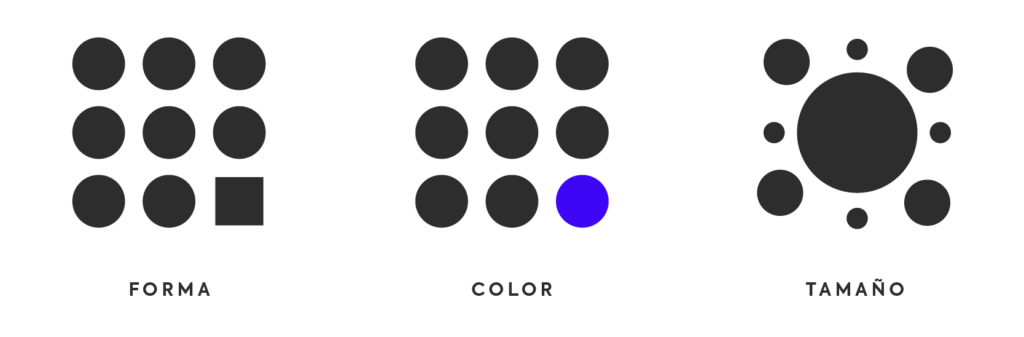
\includegraphics[width=1\linewidth,height=1\textheight]{enfasis} 

}

\caption{Unidad continuidad}\label{fig:enfasisw}
\end{figure}

\hypertarget{equilibrio-o-balance}{%
\section{Equilibrio o balance}\label{equilibrio-o-balance}}

\begin{definition}[Equilibrio]
\protect\hypertarget{def:r}{}{\label{def:r} \iffalse (Equilibrio) \fi{} }El equilibrio se basa en la organización de los elementos de modo que \textbf{nada domine en el plano o bien para que una parte pese más que la otra}.

Existen dos tipos de equilibrio: la simetría y la asimetría.
\end{definition}

\begin{itemize}
\item
  \textbf{Balance Simétrico}: se da cuando los elementos se disponen simétricamente a ambos lados de los ejes, horizontal o vertical.
\item
  \textbf{Balance Asimétrico}: se da cuando los elementos no mantienen simetría por forma, pero sí por peso visual.
\end{itemize}

The Tripled by Peter Petrov on Sketchfab

Fractal Tree3D Test by Lars Magnus Nyland on Sketchfab

\begin{figure}

{\centering 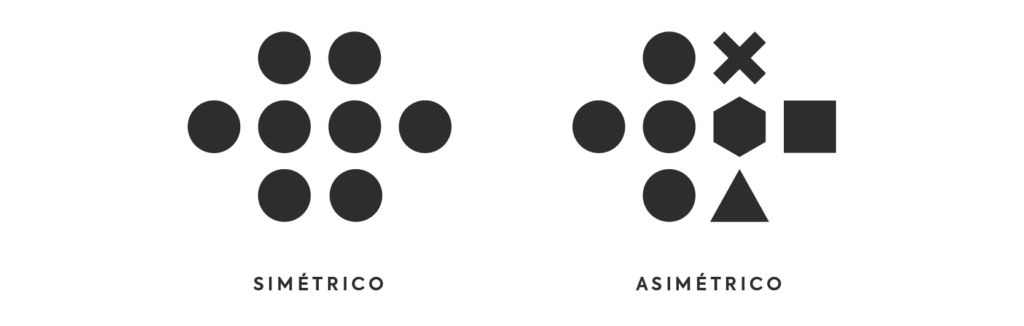
\includegraphics[width=1\linewidth,height=1\textheight]{equilibrio} 

}

\caption{Unidad continuidad}\label{fig:equilibrio}
\end{figure}

\hypertarget{ritmo-o-movimiento}{%
\section{Ritmo o movimiento}\label{ritmo-o-movimiento}}

El principio del ritmo consiste en la \textbf{repetición de elementos} con el fin de conseguir una \textbf{composición harmoniosa}. Dicha repetición puede ser \textbf{constante o alterna}, afectadas por el color, la forma, etc.

Este principio pretende expresar el movimiento en la composición y existen dos clases:

\begin{itemize}
\tightlist
\item
  \textbf{Regular}, cuando el movimiento es uniforme y constante
\item
  \textbf{Progresivo}, cuando el movimiento es alterno y varía.
\end{itemize}

El ritmo es la secuencia con que aparecen los elementos que componen el diseño: el orden, la repetición y la forma de organizarlos.

Si se usa correctamente este principio puede ser realmente muy útil para asegurar una correcta lectura de nuestro diseño.

El ritmo de una composición puede ser:

Radial: Si los elementos se disponen de forma circular
Lineal: Si la disposición de los elementos da una forma de continuidad.

\textless{}iframe title=``Fractal Thing'' frameborder=``0'' allowfullscreen mozallowfullscreen=``true'' webkitallowfullscreen=``true'' allow=``fullscreen; autoplay; vr'' xr-spatial-tracking execution-while-out-of-viewport execution-while-not-rendered web-share width:``100\%'' height=``500'' src=``\url{https://sketchfab.com/models/72576d675a3141bbbc4017e9b846bc86/embed}''\textgreater{}

Fractal Thing by Marc Vanlindt on Sketchfab

\begin{figure}

{\centering 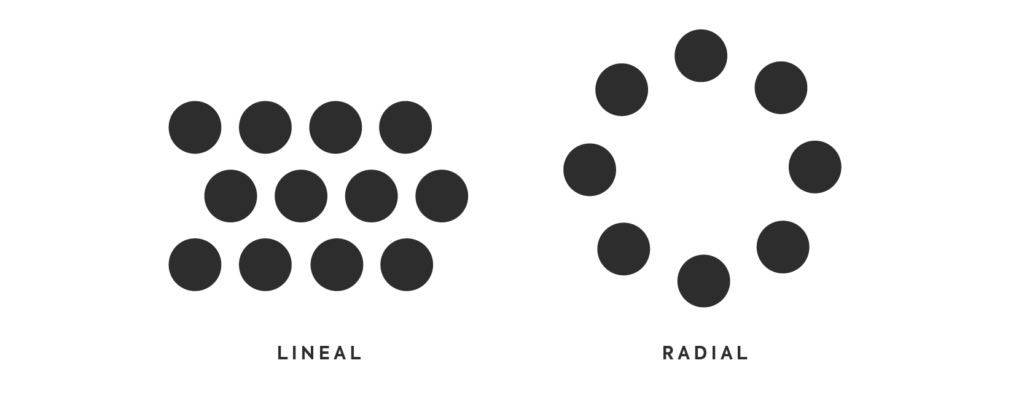
\includegraphics[width=1\linewidth,height=1\textheight]{ritmo} 

}

\caption{Ritmo regular}\label{fig:ritmo}
\end{figure}

\begin{figure}

{\centering 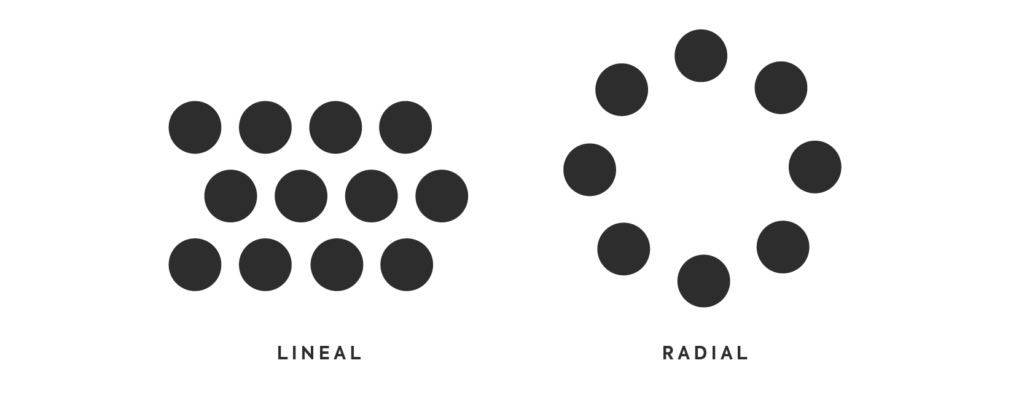
\includegraphics[width=1\linewidth,height=1\textheight]{ritmo} 

}

\caption{Ritmo regular}\label{fig:rythm}
\end{figure}

\begin{figure}

{\centering 
\includegraphics[width=1\linewidth,height=1\textheight]{ritmoo} 

}

\caption{Ritmo progresivo (secuencial)}\label{fig:rythmm}
\end{figure}

\hypertarget{proporciuxf3n-o-escala}{%
\section{Proporción o Escala}\label{proporciuxf3n-o-escala}}

El \textbf{principio de proporción} se basa en la relación del tamaño de los objetos con la composición final. La proporción nos ayuda a comunicar la \textbf{relación entre los diferentes elementos de diseño}. También puede ayudarnos a marcar como más importante alguna parte en concreto, ya que los elementos grandes captan más atención que los pequeños.

Dentro del principio de escala podemos tener en cuenta 3 subcategorías:

\begin{itemize}
\item
  \textbf{Tamaño}: cuando nos encontramos con elementos de diferentes tamaños relacionados entre sí.
\item
  \textbf{Proporción}: elementos relacionados unos con otros, en una proporción visualmente armónica.
\item
  \textbf{División}: elementos divididos en diferentes tamaños, creando todos ellos una unidad.
\end{itemize}

\begin{figure}

{\centering 
\includegraphics[width=1\linewidth,height=1\textheight]{proporcion} 

}

\caption{Ritmo regular}\label{fig:proporcion}
\end{figure}

\hypertarget{unidad}{%
\section{Unidad}\label{unidad}}

Este principio de la composición tiene lugar cuando un conjunto de \textbf{elementos} se \textbf{organizan y se relaciona entre sí}; de manera que acaban representando un \textbf{solo elemento}.

Dentro del \textbf{principio de unidad}, encontramos 3 variantes (sub-principios):

\begin{itemize}
\item
  \textbf{Repetición}: cuando el uso de un mismo elemento se utiliza repetidamente para construir la composición.
\item
  \textbf{Principio de Sucesión}: Se logra cuando se usa recurrentemente un color o un elemento donde uno de ellos mantiene el punto focal.
\item
  \textbf{Continuidad}: cuando los elementos se articulan entorno a la construcción del mensaje.
\item
  \textbf{Proximidad}: cuando se utiliza el mismo elemento para construir bloques en la composición.

  \begin{itemize}
  \item
    \textbf{Crear conexiones}: La proximidad puede generar una relación entre dos objetos, generar relevancia, jerarquía, estructurar
  \item
    \textbf{Disipar conexiones}: La proximidad también puede reflejar la carencia de relación entre elementos.
  \end{itemize}
\end{itemize}

Y no debemos olvidar que también podemos otorgar unidad mediante la armonía con el uso de colores análogos o mediante el contraste con el uso de colores complementarios, como puede verse aquí abajo.

\begin{figure}

{\centering 
\includegraphics[width=1\linewidth,height=1\textheight]{unidad1} 

}

\caption{Unidad continuidad}\label{fig:unidad1}
\end{figure}

\begin{figure}

{\centering 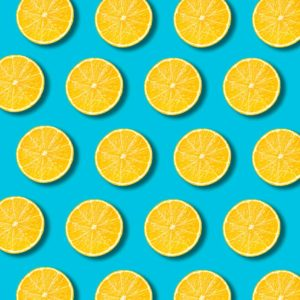
\includegraphics[width=1\linewidth,height=1\textheight]{unidad2} 

}

\caption{Unidad continuidad}\label{fig:unidad2}
\end{figure}

\begin{figure}

{\centering 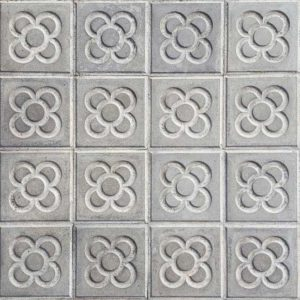
\includegraphics[width=1\linewidth,height=1\textheight]{unidad3} 

}

\caption{Unidad continuidad}\label{fig:unidad3}
\end{figure}

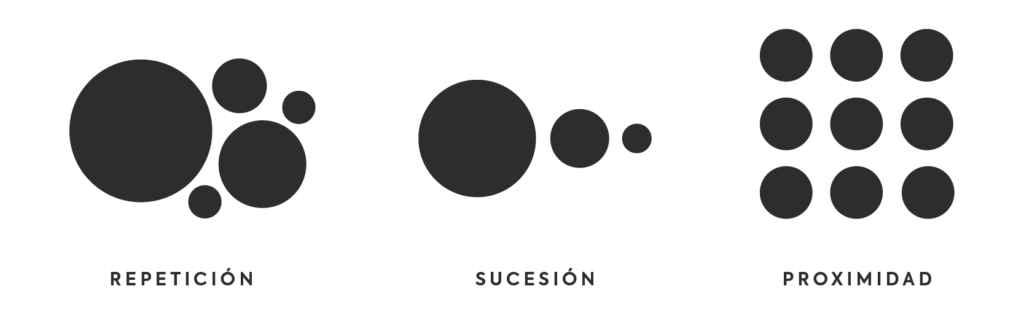
\includegraphics{unidad.png}
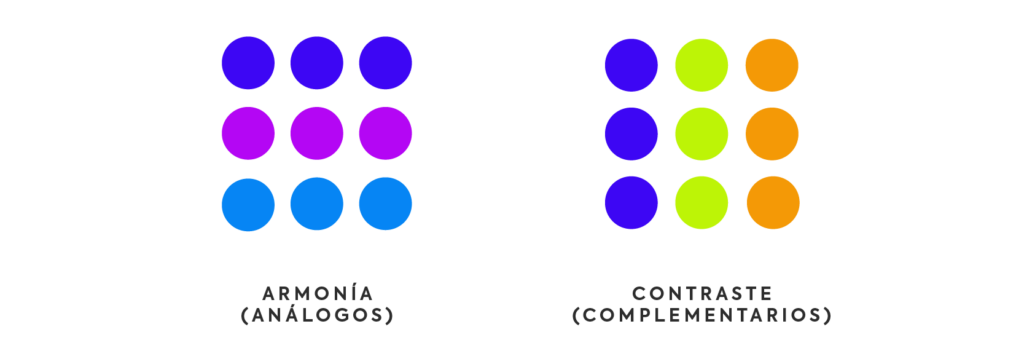
\includegraphics{unidadcolor.png}

\hypertarget{formas-tridimesionales}{%
\chapter{Formas tridimesionales}\label{formas-tridimesionales}}

\[\int_1^3\epsilon_i\]
wwwwwwwwwwwwwwwwwwwwwwwwwwl plano Here is a review of existing methods.

\begin{figure}[!ht]

{\centering \includegraphics{dibujo} 

}

\caption{Elipse}\label{fig:pressure1}
\end{figure}

\hypertarget{superficies-poliedricas}{%
\section{Superficies poliedricas}\label{superficies-poliedricas}}

www

\hypertarget{solidos-platuxf3nicos}{%
\subsection{Solidos platónicos}\label{solidos-platuxf3nicos}}

\hypertarget{los-prismas}{%
\subsection{Los prismas}\label{los-prismas}}

\hypertarget{superficies-de-revolucion-y-regladas}{%
\section{Superficies de revolucion y regladas}\label{superficies-de-revolucion-y-regladas}}

\hypertarget{superficies-curvas}{%
\section{Superficies curvas}\label{superficies-curvas}}

\hypertarget{cerradas}{%
\subsection{Cerradas}\label{cerradas}}

Esfera Elipsoide

\hypertarget{abiertas}{%
\subsection{Abiertas}\label{abiertas}}

\hypertarget{orientables}{%
\subsection{Orientables}\label{orientables}}

\hypertarget{no-orientables}{%
\subsection{No orientables}\label{no-orientables}}

\hypertarget{fractales-3d}{%
\section{Fractales 3D}\label{fractales-3d}}

\hypertarget{desarrollo-de-forma-tridimensionales}{%
\section{Desarrollo de forma tridimensionales}\label{desarrollo-de-forma-tridimensionales}}

\hypertarget{composiciuxf3n-de-formas}{%
\chapter{Composición de formas}\label{composiciuxf3n-de-formas}}

\hypertarget{operaciones-con-formas}{%
\section{Operaciones con formas}\label{operaciones-con-formas}}

\hypertarget{union}{%
\subsection{Union}\label{union}}

\begin{definition}
\protect\hypertarget{def:unnamed-chunk-1}{}{\label{def:unnamed-chunk-1} }wwwwwwwwwwwwwwwwwwwwwww
\end{definition}

\hypertarget{interseccion}{%
\subsection{Interseccion}\label{interseccion}}

\hypertarget{diferencia}{%
\subsection{Diferencia}\label{diferencia}}

\hypertarget{diferencia-simetrica}{%
\subsection{Diferencia simetrica}\label{diferencia-simetrica}}

\hypertarget{complemento}{%
\subsection{Complemento}\label{complemento}}

\hypertarget{componiendo-escenas}{%
\section{Componiendo escenas}\label{componiendo-escenas}}

\hypertarget{utilizando-software}{%
\subsection{Utilizando software}\label{utilizando-software}}

\hypertarget{el-bodegon}{%
\subsection{El bodegon}\label{el-bodegon}}

\hypertarget{la-superficie}{%
\subsection{La superficie}\label{la-superficie}}

\hypertarget{wwwwwwwwwww}{%
\subsection{wwwwwwwwwww}\label{wwwwwwwwwww}}

\hypertarget{simetruxedas}{%
\section{Simetrías}\label{simetruxedas}}

\hypertarget{simetruxeda-axial}{%
\subsection{Simetría axial}\label{simetruxeda-axial}}

\hypertarget{simetruxeda-radial-o-puntual}{%
\subsection{Simetría radial o puntual}\label{simetruxeda-radial-o-puntual}}

\hypertarget{simetruxeda-esferica}{%
\subsection{Simetría esferica}\label{simetruxeda-esferica}}

\hypertarget{simetruxeda-planar}{%
\subsection{Simetría planar}\label{simetruxeda-planar}}

\hypertarget{formas-organicas}{%
\chapter{Formas organicas}\label{formas-organicas}}

\hypertarget{geometrizacion}{%
\section{Geometrizacion}\label{geometrizacion}}

\hypertarget{redes}{%
\section{Redes}\label{redes}}

\hypertarget{geomorfologia}{%
\section{Geomorfologia}\label{geomorfologia}}

\hypertarget{fitomorfologia}{%
\section{Fitomorfologia}\label{fitomorfologia}}

\hypertarget{zoomorfologia}{%
\section{Zoomorfologia}\label{zoomorfologia}}

\hypertarget{formas-abstractas}{%
\chapter{Formas abstractas}\label{formas-abstractas}}

\hypertarget{caos-y-orden}{%
\section{Caos y orden}\label{caos-y-orden}}

\citep{bookdown2016}wwwwwww \citep{vincze2014college}

\hypertarget{ejercicios}{%
\section{Ejercicios}\label{ejercicios}}

wwwwwwwwwwwwwwwwwwwwwwwwwwwwwwwwwwww

\hypertarget{formas-matematicas}{%
\chapter{Formas Matematicas}\label{formas-matematicas}}

\begin{Shaded}
\begin{Highlighting}[]
\NormalTok{knitr}\OperatorTok{::}\KeywordTok{kable}\NormalTok{(}
  \KeywordTok{head}\NormalTok{(iris, }\DecValTok{20}\NormalTok{), }\DataTypeTok{caption =} \StringTok{'Here is a nice table!'}\NormalTok{,}
  \DataTypeTok{booktabs =} \OtherTok{TRUE}
\NormalTok{)}
\end{Highlighting}
\end{Shaded}

\begin{table}

\caption{\label{tab:nice-tab}Here is a nice table!}
\centering
\begin{tabular}[t]{rrrrl}
\toprule
Sepal.Length & Sepal.Width & Petal.Length & Petal.Width & Species\\
\midrule
5.1 & 3.5 & 1.4 & 0.2 & setosa\\
4.9 & 3.0 & 1.4 & 0.2 & setosa\\
4.7 & 3.2 & 1.3 & 0.2 & setosa\\
4.6 & 3.1 & 1.5 & 0.2 & setosa\\
5.0 & 3.6 & 1.4 & 0.2 & setosa\\
\addlinespace
5.4 & 3.9 & 1.7 & 0.4 & setosa\\
4.6 & 3.4 & 1.4 & 0.3 & setosa\\
5.0 & 3.4 & 1.5 & 0.2 & setosa\\
4.4 & 2.9 & 1.4 & 0.2 & setosa\\
4.9 & 3.1 & 1.5 & 0.1 & setosa\\
\addlinespace
5.4 & 3.7 & 1.5 & 0.2 & setosa\\
4.8 & 3.4 & 1.6 & 0.2 & setosa\\
4.8 & 3.0 & 1.4 & 0.1 & setosa\\
4.3 & 3.0 & 1.1 & 0.1 & setosa\\
5.8 & 4.0 & 1.2 & 0.2 & setosa\\
\addlinespace
5.7 & 4.4 & 1.5 & 0.4 & setosa\\
5.4 & 3.9 & 1.3 & 0.4 & setosa\\
5.1 & 3.5 & 1.4 & 0.3 & setosa\\
5.7 & 3.8 & 1.7 & 0.3 & setosa\\
5.1 & 3.8 & 1.5 & 0.3 & setosa\\
\bottomrule
\end{tabular}
\end{table}

wwwwwwwwwwwwwwwwwwwwwwwwwww

\hypertarget{funciones}{%
\section{Funciones}\label{funciones}}

wwwwwwwwww\index{wwwwwwww} \citep{vincze2014college}

\hypertarget{ejercicios-1}{%
\section{Ejercicios}\label{ejercicios-1}}

\hypertarget{appendix-apendice}{%
\appendix \addcontentsline{toc}{chapter}{\appendixname}}


Temas de reforzamiento o conocimientos preliminares que son necesarias para entender el contenido.

\hypertarget{trasformaciones}{%
\chapter{Trasformaciones}\label{trasformaciones}}

Se refiere a las transformaciones o modificaciones que pueden sufrir las formas, es decir los achatamientos, las elongaciones los cambios de posición etc., mediante la manipulación de los puntos pertenecientes a la forma.

\begin{definition}[Transformación]
\protect\hypertarget{def:transformacion}{}{\label{def:transformacion} \iffalse (Transformación) \fi{} }Una transformacion es el proceso de modificar una forma covirtiendola en otra
\end{definition}

\hypertarget{trasformaciones-elementales}{%
\section{Trasformaciones elementales}\label{trasformaciones-elementales}}

En esta sección se trata sobre la trasformaciones básicas que son la traslación, la rotación, la reflexión y la homotescia o escala

\hypertarget{traslacion}{%
\subsection{Traslacion}\label{traslacion}}

\begin{definition}[Traslación]
\protect\hypertarget{def:traslacion}{}{\label{def:traslacion} \iffalse (Traslación) \fi{} }La traslacion de un objeto, consiste en mover todos los puntos del objeto en el espacio 2D o 3D en una solo dirección, un solo sentido y a una distancia determinada.
\end{definition}

\begin{example}
\protect\hypertarget{exm:unnamed-chunk-2}{}{\label{exm:unnamed-chunk-2} }Sea figura (\ref{fig:Doge}) la derección de \(37^\circ\), el sentido indicada por la flecha y la distancia 5 unidades.
\end{example}

www

\begin{figure}

{\centering 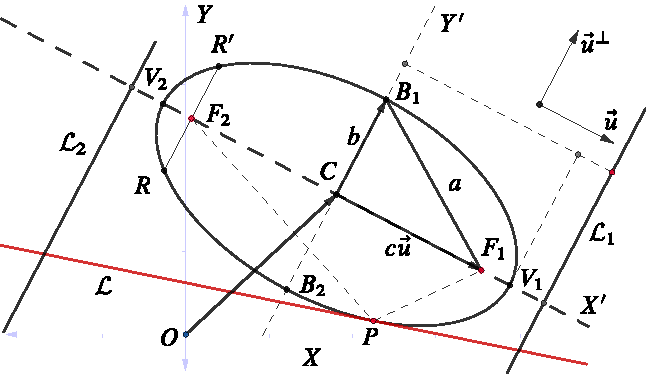
\includegraphics{elipse} 

}

\caption{Hola}\label{fig:Doge}
\end{figure}

\begin{example}
\protect\hypertarget{exm:unnamed-chunk-3}{}{\label{exm:unnamed-chunk-3} }www wwwwwwwwwwww wwwwwwwwwwwwwww
\end{example}

En la escala u homotescia también existen procedimientos de proporción \ref{fig:Doge}

\hypertarget{rotacion}{%
\subsection{Rotacion}\label{rotacion}}

\begin{definition}[Traslación]
\protect\hypertarget{def:rotacion}{}{\label{def:rotacion} \iffalse (Traslación) \fi{} }La traslacion es el proceso de mover todos los puntos de un objeto en el espacio 2D o 3D en una solo dirección y sentido a una distancia determinada
\end{definition}

\hypertarget{reflexiuxf3n}{%
\subsection{Reflexión}\label{reflexiuxf3n}}

La traslacion es el proceso de mover todos los puntos de un objeto en el espacio 2D o 3D en una solo dirección y sentido a una distancia determinada

\hypertarget{homotescia}{%
\subsection{Homotescia}\label{homotescia}}

La traslacion es el proceso de mover todos los puntos de un objeto en el espacio 2D o 3D en una solo dirección y sentido a una distancia determinada

\hypertarget{trasformaciones-topoluxf3gicas}{%
\section{Trasformaciones topológicas}\label{trasformaciones-topoluxf3gicas}}

La traslacion es el proceso de mover todos los puntos de un objeto en el espacio 2D o 3D en una solo dirección y sentido a una distancia determinada

\hypertarget{homeomofismo}{%
\subsection{Homeomofismo}\label{homeomofismo}}

La traslacion es el proceso de mover todos los puntos de un objeto en el espacio 2D o 3D en una solo dirección y sentido a una distancia determinada

\hypertarget{homomorfismo}{%
\subsection{Homomorfismo}\label{homomorfismo}}

La traslacion es el proceso de mover todos los puntos de un objeto en el espacio 2D o 3D en una solo dirección y sentido a una distancia determinada \citep{xie2015}

\hypertarget{isomorfismo}{%
\subsection{Isomorfismo}\label{isomorfismo}}

\hypertarget{isometruxeda}{%
\subsection{Isometría}\label{isometruxeda}}

\hypertarget{centro-de-masa}{%
\chapter{Centro de masa}\label{centro-de-masa}}

\hypertarget{centro-de-masa-de-objetos-2d}{%
\section{Centro de masa de objetos 2D}\label{centro-de-masa-de-objetos-2d}}

\hypertarget{metodos-matematicos}{%
\subsection{Metodos matematicos}\label{metodos-matematicos}}

\hypertarget{metodos-tecnicos}{%
\subsection{Metodos tecnicos}\label{metodos-tecnicos}}

\hypertarget{muxe9todo-del-borde-de-la-mesa}{%
\subsubsection{Método del borde de la mesa}\label{muxe9todo-del-borde-de-la-mesa}}

\hypertarget{muxe9todo-de-la-plomada}{%
\subsubsection{Método de la plomada}\label{muxe9todo-de-la-plomada}}

\hypertarget{centro-de-masa-de-objetos-3d}{%
\section{Centro de masa de objetos 3D}\label{centro-de-masa-de-objetos-3d}}

\hypertarget{metodos-matematicos-1}{%
\subsection{Metodos matematicos}\label{metodos-matematicos-1}}

\hypertarget{metodos-tecnicos-1}{%
\subsection{Metodos tecnicos}\label{metodos-tecnicos-1}}

\hypertarget{muxe9todo-de-las-secciones}{%
\subsubsection{Método de las secciones}\label{muxe9todo-de-las-secciones}}

\hypertarget{muxe9todo-de-la-plomada-1}{%
\subsubsection{Método de la plomada}\label{muxe9todo-de-la-plomada-1}}

\bibliography{book.bib,packages.bib}

\printindex

\end{document}
